%-------------------------------------------------------------------------------
%	CAPITOLO 27
%-------------------------------------------------------------------------------

\chapter{Boari - Il secchio e il pozzo - L'ipepacuana}
\begin{wrapfigure}{R}{0.2\textwidth}
  \vspace{-1.2cm}
  \begin{center}
    
\includegraphics[width=0.2\textwidth]{Boari}
  \end{center}
  \vspace{-0.5cm}
\end{wrapfigure}
\index[Personaggi]{Boari Attilio (farmacista)}Era una curiosa macchietta ed ancora un più curioso carattere. Volubile, senza idee, deve essere un benemerito del paese per il benefico lascito al ricovero\footnote{\textbf{Attilio Boari}, morendo nel 1903, lasciò la sua eredità ad un ricovero per poveri vicino al vecchio cimitero, oggi via 2 giugno. A lui è oggi intitolata una via, ad Alfonsine. Dopo la sua morte, vi furono molte delibere per decidere come utilizzare al meglio l'eredità. }. La fortuna del ricovero fu che il Boari morì, poco dopo il testamento, senza il tempo di poterlo disfare. Originario di Monesterolo\footnote{Monasterolo di Castello, Bergamo}, venne qui come farmacista, sposò la Signora \index[Personaggi]{Salvatori Giovanna}Giovanna Salvatori, rimase vedovo e senza figlio, abbastanza vecchiotto... e per rifarsi dalla tutela della moglie ebbe e presunse di avere varie conquiste... a suon di marenghi\footnote{Soldi}.\\
\indent Sapeva fare il chinino\footnote{Preparato a base di chinina, alcaloide estratto dalla corteccia di china, una pianta sudamericana. Il chinino serviva come farmaco, ma poteva essere usato anche per fare un liquore}, dell'ottima polpa di tamarindo e dei rosali che regalava in piccole bottiglie agli amici per le feste.\\
\indent Per calcolare i crediti della farmacia, a fine anno, pesava le ricette... e dalla risultanza diceva <<tanti amici e tanto da incassare!>>\\
\indent Si mescolava sempre ai giovani, si riteneva nella vedovanza uno scapolo ed i burloni gli cantavano:\\\\
\textcal \Huge
	\centerline{Il vecchietto cerca moglie}
	\centerline{vuole marito la ragazza}
	\centerline{l'uno freme e l'altro è pazzo}
	\centerline{ecc...}
\normalfont \normalsize\\

Un giorno gli chiedemmo perché non aveva avuto figli.\\
\indent Rispose: <<La secchia non arrivava in fondo al pozzo...>> (di S. Patrizio\footnote{Il pozzo di San Patrizio si trova in Umbria ed è profondo 53,13 metri} si crede!)\\
\indent Si addormentava d'estate a gola aperta su uno sgabello a sdraio in farmacia, si svegliava quando era ben coperto e punzecchiato si alzava ed aveva la velleità di andare... a filare. \\
\indent Per i begli occhi della .\:.\:.\footnote{Nome mancante} era geloso del \index[Personaggi]{Gamberini Dr. Giulio}Dr. Gamberini\footnote{\textbf{Dr. Giulio Gamberini}, primario dell'ospedale di Alfonsine dal 1876. L'ospedale venne poi intitolato a suo nome.} col quale venne alle mani e non gliela perdonò più. \\
\indent Alla sera si sbarrava nella camera da letto con una spranga di legno, passeggiava con uno di quei pai\footnote{Paia} di scarpe che facevano cric crac, mormorava <<Cat vègna un azidènt sèc\footnote{<<Che ti venga un accidente secco>>}>> (quasi sempre alludeva al \index[Personaggi]{Gamberini Dr. Giulio}Dr. Gamberini) e giù una trombettata\footnote{Pernacchia}, e poi <<te vigliac\footnote{<<Tu vigliacco...>>}...>> e così durava delle ore a sfogare la sua gelosia.\\

\indent Un giorno gli facemmo uno scherzo. Erano passate delle pecore che avevano seminate certe pillole\footnote{Le pecore, pascolando avevano lasciato sul terreno escrementi tondi come palline}. Ne raccogliemmo una buona dose, secrate ed infarinate le mettemmo in una scatola bella, tutta argentata, e poi chiedemmo al nostro \index[Personaggi]{Boari Attilio (farmacista)}Boari, complice l'aiutante farmacista: <<Abbiamo trovato questa scatola, che pillole sono?>>\\
\indent Boari ne prese una, la fiutò, fece una smorfia, poi se la sfregò sulla punta della lingua ed in furia emise il responso: <<L'è ipepacuana\footnote{L'Ipecacuana è un arbusto originario dell'India, coltivato anche nel Sud America ed in Malesia ed è un emetico (provoca il vomito)}>>\\
\indent Non poté mai scoprire la burla altrimenti permaloso com'era non ce l'avrebbe perdonata.

\vspace{1cm}
\centerline{\rule{1.5cm}{0.4pt}}
\vspace{1cm}

 \begin{figure}[htb]
    \centering
    %\vspace{-0.7cm}
    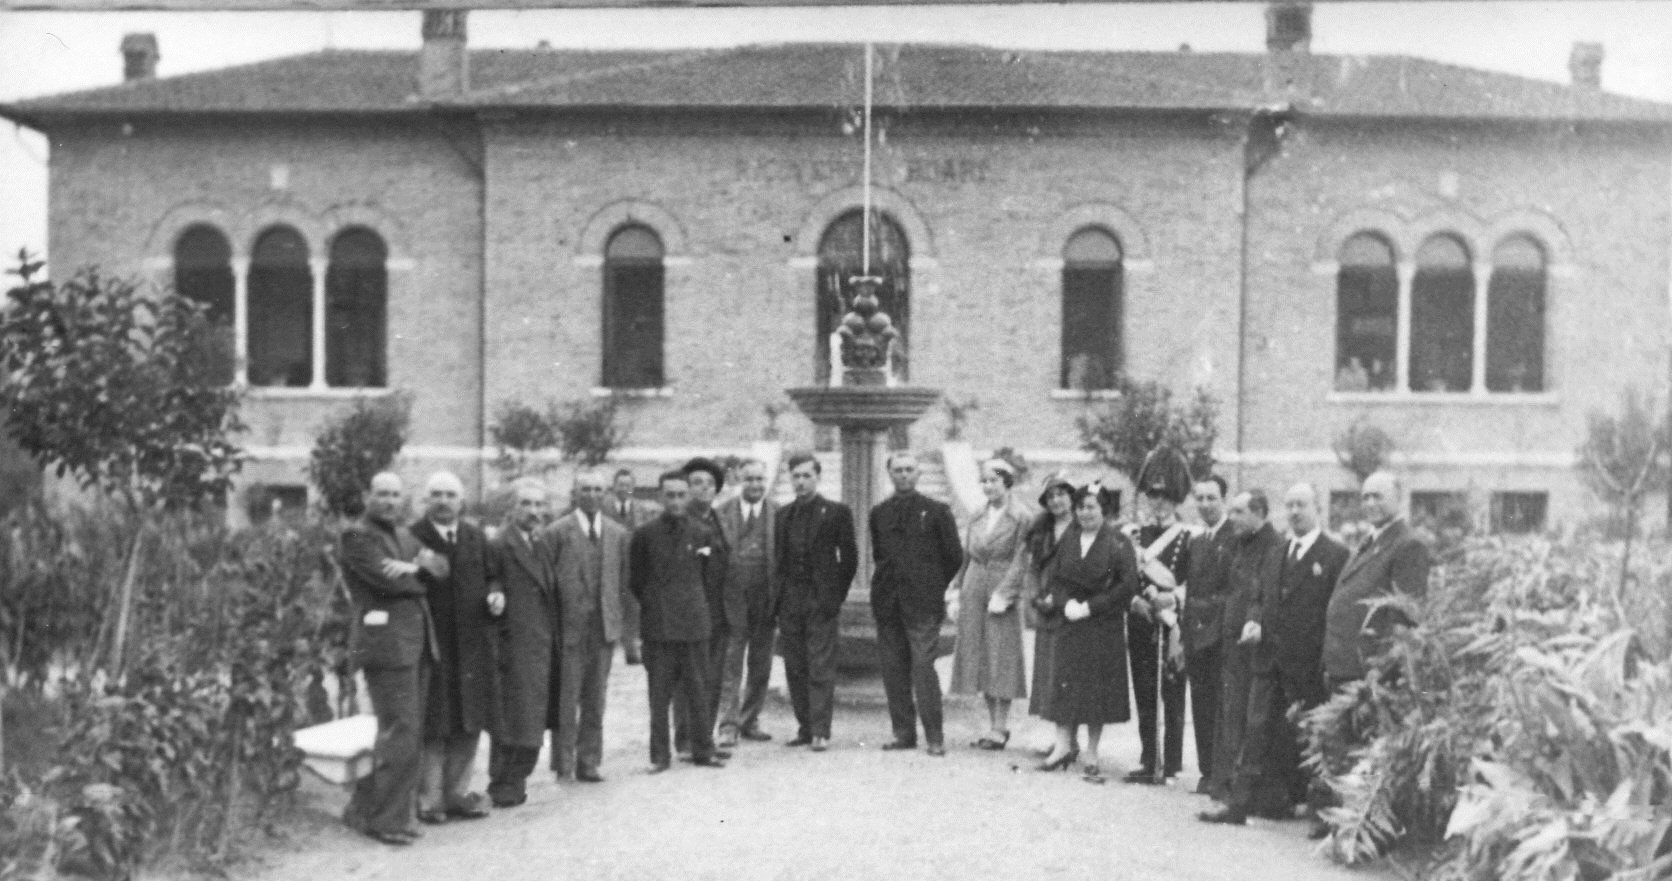
\includegraphics[width=\textwidth]{RicoveroBoari}
    \caption*{Il ricovero \index[Luoghi]{Ricovero A. Boari}A. Boari in via \index[Luoghi]{Reale (via)}Reale, vicino all'Ospedale, terminati entrambi nel 1930. Tra le persone presenti nella foto si riconoscono  \index[Personaggi]{Meruzzi dott. Cassiano}Meruzzi Cassiano, il secondo da sinistra e \index[Personaggi]{Marini Giuseppe}Marini Giuseppe, il primo da destra.\label{fig:RicoveroBoari}}
    %\vspace{-0.3cm}
\end{figure}
